\chapter{Проектирование и реализация прототипа}

\section{Анализ требований к функциональному прототипу}

Прототип интегрированной экспертной системы для диагностики и отладки процесса выращивания дынь в полевых условиях должен иметь два режима функционирования: режим консультации и режим имитации. Режим консультации предназначен для агронома. Режим имитации предназначен для осуществления имитационного эксперимента специалистом по имитационному моделированию.

В рамках каждого режима функционирования рассматриваемый прототип должен удовлетворять следующим требованиям:

Для режима консультации:
\begin{itemize}
    \item Выдавать рекомендации действий агроному.
\end{itemize}

Для режима имитации:
\begin{itemize}
    \item Отображать текущие значения показателей датчиков.
    \item Предоставлять возможность задания начальных значений имитационной модели.
\end{itemize}

\section{Общая архитектура, состав и структура прототипа ИЭС}

Реализация прототипа динамической ИЭС диагностики и отладки выращивания дынь в полевых условиях производилась с использованием инструментального средства – системы G2. Таким образом, при проектировании архитектуры динамической ИЭС учитывались не только требования к разрабатываемому прототипу, но и возможности инструментального средства G2.

% Рис. 4. Архитектура прототипа динамической ИЭС
% \begin{figure}[h]
%     \centering
%     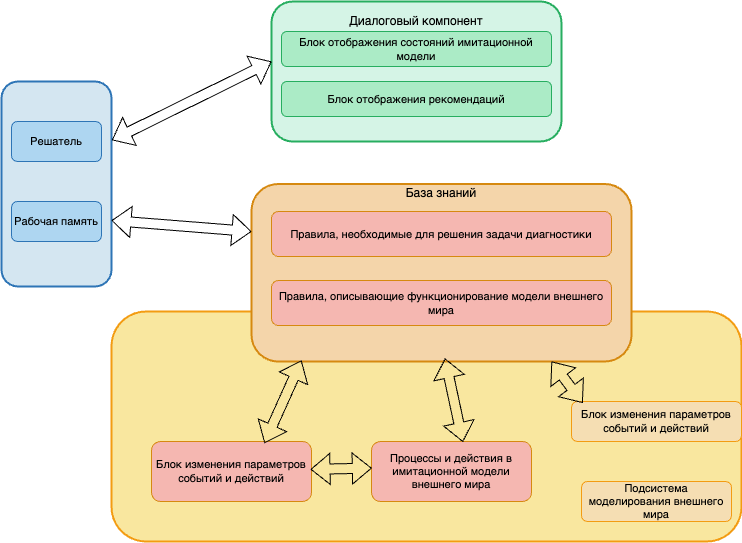
\includegraphics[width=0.8\linewidth]{img/architecture.png} % Замените на путь к вашему изображению
%     \caption{Архитектура прототипа динамической ИЭС}
%     \label{fig:architecture}
% \end{figure}

Основными архитектурными компонентами являются:
\begin{itemize}
    \item Рабочая память. Для представления рабочей памяти был выбран способ с объектом БЗ на отдельном рабочем пространстве с целью ускорения отладки путем визуального наблюдения за состоянием объектов в памяти;
    \item Решатель. При создании прототипа динамической ИЭС с помощью средств G2 используется стандартный механизм вывода в G2. Стратегия вывода – прямой вывод;
    \item Диалоговый компонент обеспечивает выдачу рекомендации о необходимости принятия мер безопасности.
    \item Подсистема моделирования внешнего мира. Для построения подсистемы моделирования внешнего мира используются методы и средства имитационного моделирования.
    \item База знания, содержащая правила двух типов:
    \begin{itemize}
        \item Правила, использующиеся для решения задач рассматриваемой проблемной области;
        \item Правила, описывающие функционирование имитационной модели;
    \end{itemize}
\end{itemize}

\section{Построение БЗ и стратегии вывода}

Исходя из архитектуры прототипа ДИС, правила БЗ делятся на две группы: правила, использующиеся для решения задачи, и правила подсистемы моделирования внешнего мира. В качестве стратегии вывода используется прямой вывод.

\section{Построение макета прототипа ИЭС}

Прототип интегрированной экспертной системы “диагностика процесса выращивания дынь в полевых условиях” имеет два режима функционирования: режим консультации и режим имитации. Вследствие отсутствия возможности построения прототипа ИЭС средствами G2 было принято решение представить макет системы “диагностика процесса выращивания дынь в полевых условиях”. Макет прототипа ИЭС на момент запуска представлен на рисунке 5.

% Рис. 5. Макет прототип ИЭС на момент запуска
% \begin{figure}[h]
%     \centering
%     \includegraphics[width=0.8\linewidth]{img/mockup_start.png} % Замените на путь к вашему изображению
%     \caption{Макет прототипа ИЭС на момент запуска}
%     \label{fig:mockup_start}
% \end{figure}

% Рис.5. Макет окна на момент запуска (дублируется, не включаем)

Макет прототипа ИЭС в режиме имитации представлен на рисунке 6.

% Рис. 6. Макет прототипа в режиме имитации
% \begin{figure}[h]
%     \centering
%     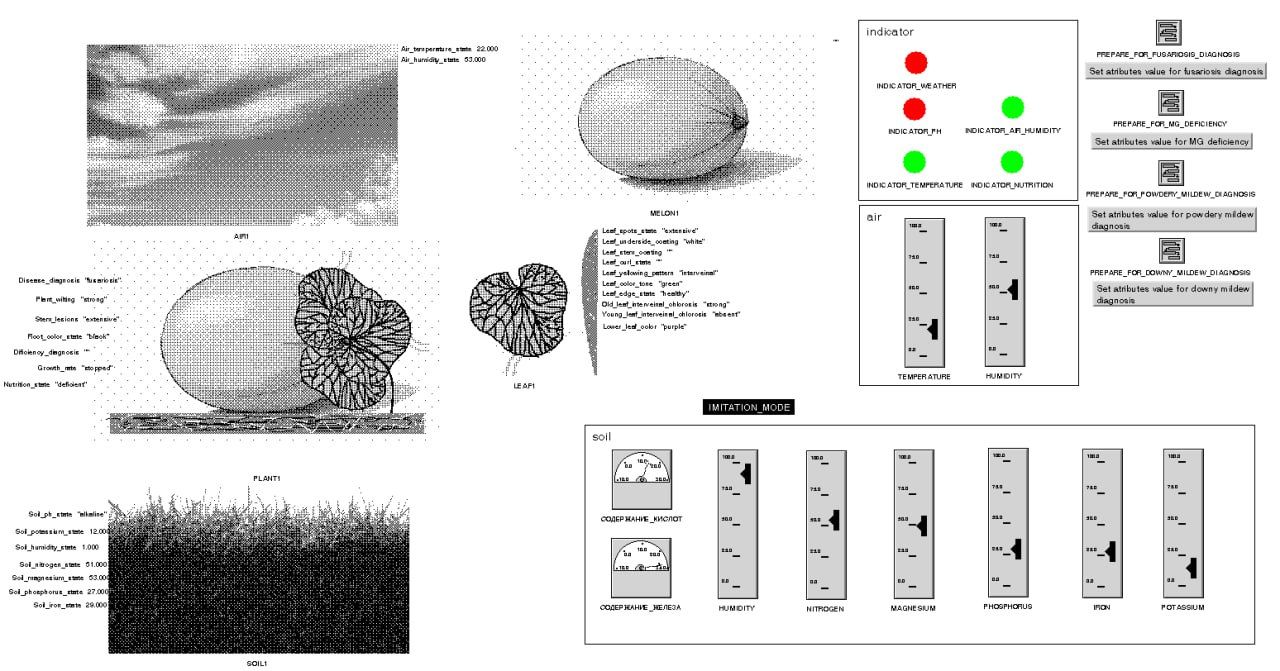
\includegraphics[width=0.8\linewidth]{img/mockup_simulation.png} % Замените на путь к вашему изображению
%     \caption{Макет прототипа в режиме имитации}
%     \label{fig:mockup_simulation}
% \end{figure}

Макет панель управления показателями представлен на рисунке 7.

% Рис. 7. Панель управления показателями
% \begin{figure}[h]
%     \centering
%     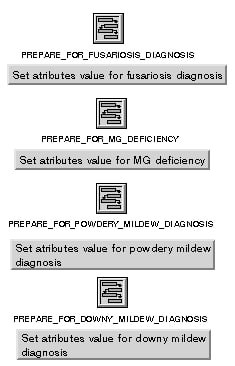
\includegraphics[width=0.8\linewidth]{img/mockup_control_panel.png} % Замените на путь к вашему изображению
%     \caption{Панель управления показателями}
%     \label{fig:mockup_control_panel}
% \end{figure}

Макет прототипа ИЭС в режиме консультации представлен на рисунке 8.

% Рис.8. Макет прототипа ИЭС в режиме консультации
% \begin{figure}[h]
%     \centering
%     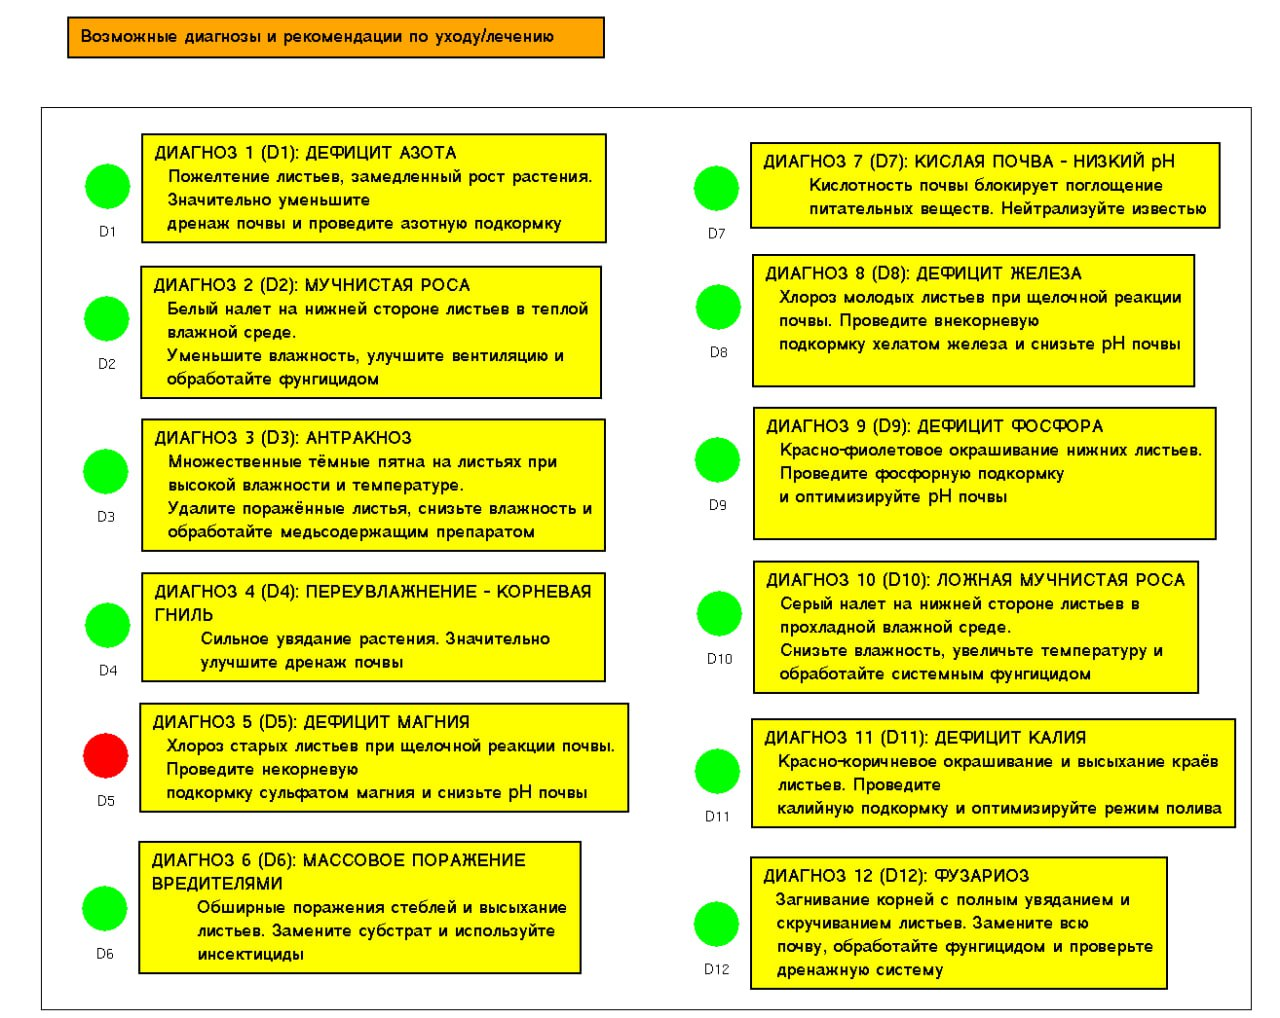
\includegraphics[width=0.8\linewidth]{img/mockup_consultation.png} % Замените на путь к вашему изображению
%     \caption{Макет прототипа ИЭС в режиме консультации}
%     \label{fig:mockup_consultation}
% \end{figure}
